\documentclass[14pt,a4paper]{scrreprt}

\usepackage{cmap}
\usepackage[T1]{fontenc} 
\usepackage[utf8]{inputenc}
\usepackage[english,russian]{babel}

\usepackage{caption}
\usepackage{subcaption}

\usepackage{float}

\usepackage{enumitem}

\usepackage{graphicx}
\usepackage{multirow}


\usepackage{pgfplots}
\pgfplotsset{compat=newest}
\usepgfplotslibrary{units}

\usepackage{longtable}

\usepackage{caption}
\captionsetup{labelsep=endash}
\captionsetup[figure]{name={Рисунок}}
\captionsetup[subtable]{labelformat=simple}
\captionsetup[subfigure]{labelformat=simple}
\renewcommand{\thesubtable}{\text{Таблица }\arabic{chapter}\text{.}\arabic{table}\text{.}\arabic{subtable}\text{ --}}
\renewcommand{\thesubfigure}{\text{Рисунок }\arabic{chapter}\text{.}\arabic{figure}\text{.}\arabic{subfigure}\text{ --}}


\usepackage{textcomp}

\usepackage{amsmath}
\usepackage{amsfonts}
\usepackage{array}

\usepackage{geometry}
\geometry{left=30mm}
\geometry{right=15mm}
\geometry{top=20mm}
\geometry{bottom=20mm}
\geometry{foot=1.7cm}

\usepackage{titlesec}
\titleformat{\section}
{\normalsize\bfseries}
{\thesection}
{1em}{}
\titlespacing*{\chapter}{0pt}{-30pt}{8pt}
\titlespacing*{\section}{\parindent}{*4}{*4}
\titlespacing*{\subsection}{\parindent}{*4}{*4}

% Маркировка для списков
\def\labelitemi{$\circ$}
\def\labelitemii{$*$}


\usepackage{setspace}
\onehalfspacing % Полуторный интервал

\frenchspacing
\usepackage{indentfirst} % Красная строка

\usepackage{titlesec}
\usepackage{xcolor}
% Названия глав
\titleformat{\section}{\normalsize\textmd}{\thesection}{1em}{}

\definecolor{gray35}{gray}{0.35}

\newcommand{\hsp}{\hspace{20pt}} % длина линии в 20pt

\titleformat{\chapter}[hang]{\Huge}{\textcolor{gray35}{\thechapter.}\hsp}{0pt}{\Huge\textmd}

\titleformat{\section}{\Large}{\textcolor{gray35}\thesection}{20pt}{\Large\textmd}
\titleformat{\subsection}{\Large}{\thesubsection}{20pt}{\Large\textmd}
\titleformat{\subsubsection}{\normalfont\textmd}{}{0pt}{}

% Настройки введения

\addtocontents{toc}{\setcounter{tocdepth}{2}}
\addtocontents{toc}{\setcounter{secnumdepth}{1}}

\usepackage{tocloft,lipsum,pgffor}

\addtocontents{toc}{~\hfill\textnormal{Страница}\par}

\renewcommand{\cftpartfont}{\normalfont\textmd}

\addto\captionsrussian{\renewcommand{\contentsname}{Содержание}}
\renewcommand{\cfttoctitlefont}{\Huge\textmd}

\renewcommand{\cftchapfont}{\normalfont\normalsize}
\renewcommand{\cftsecfont}{\normalfont\normalsize}
\renewcommand{\cftsubsecfont}{\normalfont\normalsize}
\renewcommand{\cftsubsubsecfont}{\normalfont\normalsize}

\renewcommand{\cftchapleader}{\cftdotfill{\cftdotsep}}

\usepackage{listings}
\usepackage{xcolor}

\usepackage[pdftex]{hyperref} % Гиперссылки
\hypersetup{hidelinks}

% Листинги 
\usepackage{listings}

\definecolor{darkgray}{gray}{0.15}

\definecolor{teal}{rgb}{0.25,0.88,0.73}
\definecolor{gray}{rgb}{0.5,0.5,0.5}
\definecolor{b-red}{rgb}{0.88,0.25,0.41}
\definecolor{royal-blue}{rgb}{0.25,0.41,0.88}

\usepackage{listings}
\lstset{
	aboveskip=3mm,
	belowskip=3mm,
	frame=tb,
	frame=single,
	basicstyle=\footnotesize\ttfamily,
	numberstyle=\tiny\color{gray},
	keywordstyle=\color{royal-blue},
	commentstyle=\color{gray35},
	stringstyle=\color{b-red},
	numbers=left,
	numbersep=5pt,
	numberstyle=\tiny,
	showstringspaces=false, 
	captionpos=t,
	tabsize=4,
	language=C
}

% какой то сложный кусок со стак эксчейндж для квадратных скобок
\makeatletter
\newenvironment{sqcases}{%
	\matrix@check\sqcases\env@sqcases
}{%
	\endarray\right.%
}
\def\env@sqcases{%
	\let\@ifnextchar\new@ifnextchar
	\left\lbrack
	\def\arraystretch{1.2}%
	\array{@{}l@{\quad}l@{}}%
}
\makeatother

% и для матриц
\makeatletter
\renewcommand*\env@matrix[1][\arraystretch]{%
	\edef\arraystretch{#1}%
	\hskip -\arraycolsep
	\let\@ifnextchar\new@ifnextchar
	\array{*\c@MaxMatrixCols c}}
\makeatother


\begin{document}

\begin{titlepage}
	
	\newgeometry{left=2cm, right=2cm, top=2.5cm, bottom=2.5cm}
	\fontsize{12pt}{12pt}\selectfont
	
	\noindent \begin{minipage}{0.13\textwidth}
		
\includegraphics[width=\linewidth]{assets/bmstu-logo.png}
	\end{minipage}
	\noindent\begin{minipage}{0.85\textwidth}\centering
		\textbf{\textsc{Министерство науки и высшего образования Российской Федерации}}\\
		\textbf{\textsc{Федеральное государственное бюджетное образовательное 	учреждение высшего образования}}\\
		\textbf{\textsc{Московский государственный технический университет имени 	Н.Э.~Баумана}}\\
		\textbf{\textsc{(национальный исследовательский университет)}}\\
		\textbf{\textsc{(МГТУ им. Н.Э. Баумана)}}\\
	\end{minipage}
	
	\noindent\rule{18cm}{1.5pt}
	
	\vspace{8mm}
	
	\noindent\textnormal{ФАКУЛЬТЕТ}\hspace{5mm} \underline{\textnormal{~~~~~~~~~~~~~~~~~~«Информатика и системы управления»~~~~~~~~~~~~~~~~~~}} \newline\newline
	\textnormal{КАФЕДРА}\hspace{5mm} \underline{\textnormal{~~«Программное обеспечение ЭВМ и информационные технологии»~~}}
	\newline\newline
	\textnormal{НАПРАВЛЕНИЕ ПОДГОТОВКИ}\hspace{5mm} \underline{\textnormal{~~~~~~«09.03.04 Программная инженерия»~~~~~~~~}}
	
	\vspace{2.5cm}
	
	\begin{center}
		\Large\textbf{\textsc{ОТЧЕТ}}\\
		\Large\textbf{\textsc{ПО ЛАБОРАТОРНОЙ РАБОТЕ №5}}\\
	\end{center}
	
	\vspace{1cm}
	
	\noindent\textnormal{Название:} \hspace{15mm} \underline{\textnormal{~~~~~Буферизованный и не буферизованный ввод-вывод~~~~~~~}}\noindent
	
	\vspace{1.3cm}
	
	\noindent\textnormal{Дисциплина:} \hspace{10mm} \underline{\textnormal{~~~~~~~~~~~~~~~~~~~~~~~~~~Операционные системы~~~~~~~~~~~~~~~~~~~~~~~~}}\noindent
	
	\vspace{1.5cm}
	
	\noindent\textnormal{Студент} \hspace{17mm}
	\underline{\textnormal{{~~~~ИУ7-64Б~~~}}}
	\hspace{20mm}
	\underline{\textnormal{\hphantom{~~~~~~~~~~~~~~~~~~~~~~~~~~~}}} \hspace{10mm}
	\underline{\textnormal{~~~С. Д. Параскун~~~~}}
	
	\vspace{2mm}
	\noindent\textnormal{\hphantom{Студент}} \hspace{23mm}\noindent
	\fontsize{8pt}{8pt}
	\textnormal{Группа}\hspace{40mm}\textnormal{Подпись, дата} \hspace{28mm}\noindent\textnormal{И. О. Фамилия}
	
	\vspace{0.5cm}
	
	\fontsize{12pt}{12pt}\selectfont
	\noindent\textnormal{Преподаватель} \hspace{52mm}
	\underline{\textnormal{\hphantom{~~~~~~~~~~~~~~~~~~~~~~~~~~~}}} \hspace{10mm}
	\noindent\underline{\textnormal{~Н. Ю. Рязанова~}}
	
	\vspace{2mm}
	\noindent\textnormal{\hphantom{Студент}} \hspace{17mm}\noindent
	\fontsize{8pt}{8pt}
	\hphantom{Группа}\hspace{43mm}\textnormal{Подпись, дата} \hspace{28mm}\noindent\textnormal{И. О. Фамилия}
	
	\vspace{2cm}
	
	\fontsize{12pt}{12pt}\selectfont
	
	\begin{center}
		\vfill
		Москва, ~\the\year
		~г.
	\end{center}
	\restoregeometry

\end{titlepage}


\thispagestyle{empty}

\chapter{Используемые структуры данных}

В данной лабораторной анализировалась работа системного вызова open() для версии ядра 5.17.5.

\begin{lstlisting}[caption=Структура open\_flags]
struct open_flags {
	int open_flag;
	umode_t mode;
	int acc_mode;
	int intent;
	int lookup_flags;
};
\end{lstlisting}

\begin{lstlisting}[caption=Структура filename]
struct filename {
	const char *name;	/* pointer to actual string */
	const __user char *uptr;	/* original userland pointer */
	int refcnt;
	struct audit_names *aname;
	const char iname[];
};
\end{lstlisting}

\begin{lstlisting}[caption=Структура nameidata]
struct nameidata {
	struct path	path;
	struct qstr	last;
	struct path	root;
	struct inode	*inode; /* path.dentry.d_inode */
	unsigned int	flags, state;
	unsigned	seq, m_seq, r_seq;
	int		last_type;
	unsigned	depth;
	int		total_link_count;
	struct saved {
		struct path link;
		struct delayed_call done;
		const char *name;
		unsigned seq;
	} *stack, internal[EMBEDDED_LEVELS];
	struct filename	*name;
	struct nameidata *saved;
	unsigned	root_seq;
	int		dfd;
	kuid_t		dir_uid;
	umode_t		dir_mode;
} __randomize_layout;
\end{lstlisting}

\chapter{Схемы алгоритмов}

\begin{figure}[H]
	\begin{center}
		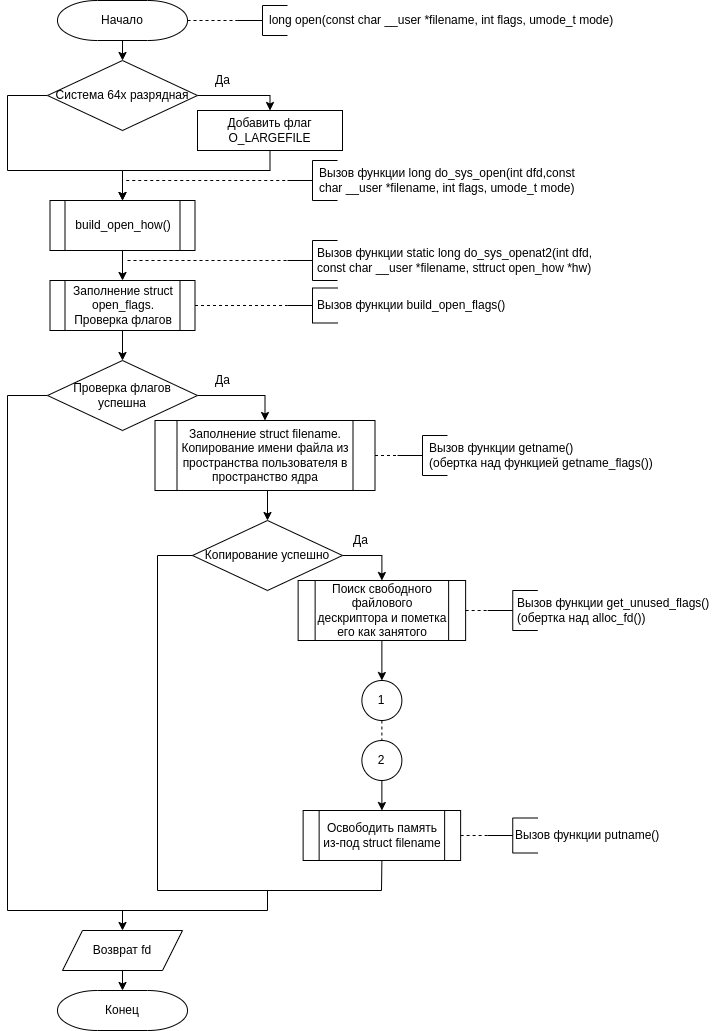
\includegraphics[scale=0.58]{assets/open-1.png}
	\end{center}
	\caption{Схема алгоритма работы системного вызова open()}
\end{figure}

\begin{figure}[H]
	\begin{center}
		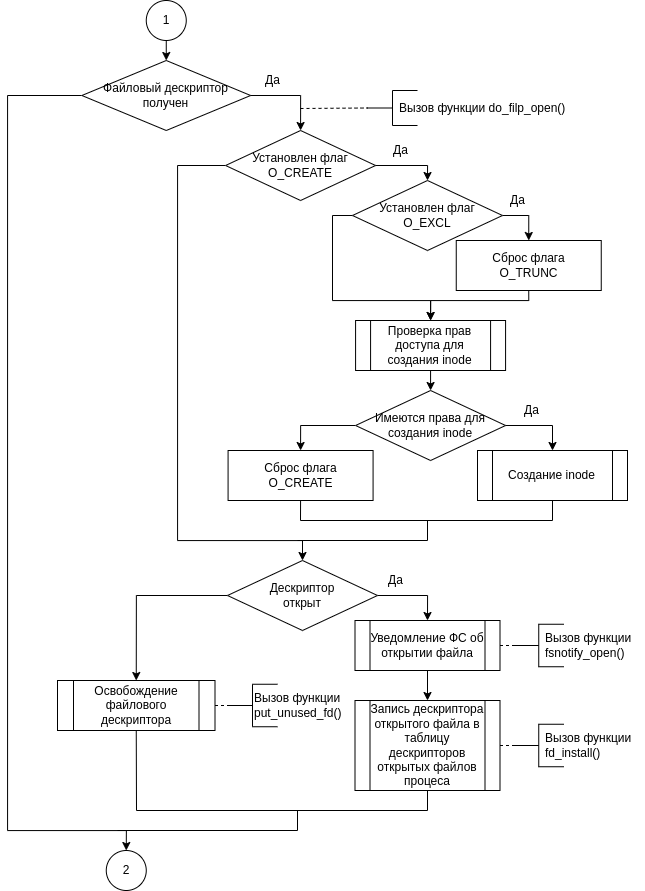
\includegraphics[scale=0.7]{assets/open-2.png}
	\end{center}
	\caption{Схема алгоритма работы системного вызова open() (продолжение)}
\end{figure}

\begin{figure}[H]
	\begin{center}
		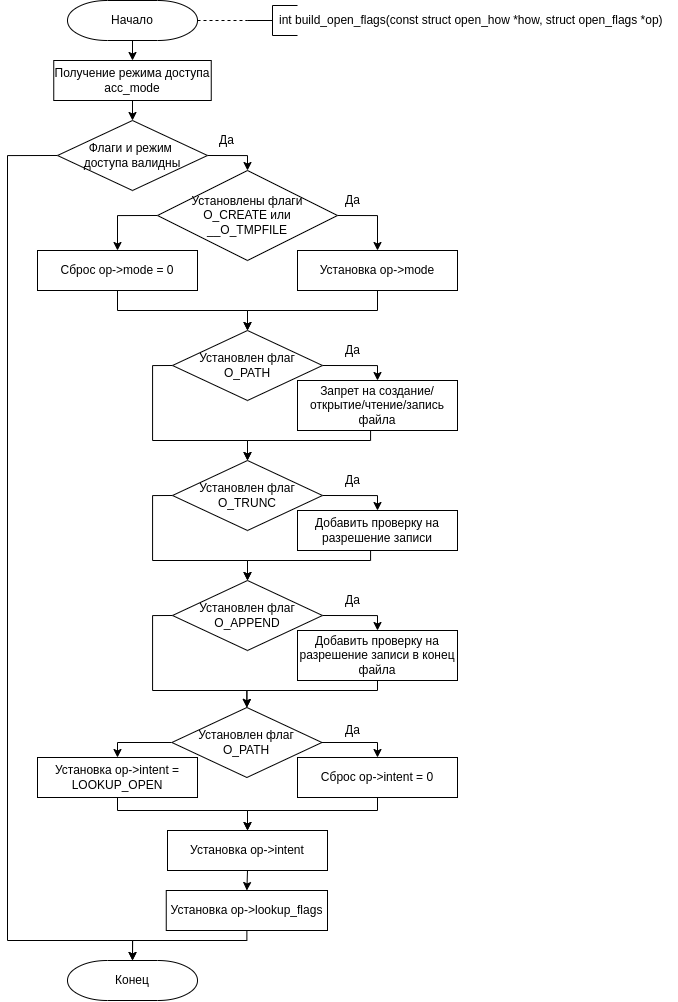
\includegraphics[scale=0.7]{assets/build_open_flags.png}
	\end{center}
	\caption{Схема алгоритма работы функции build\_open\_flags()}
\end{figure}

\begin{figure}[H]
	\begin{center}
		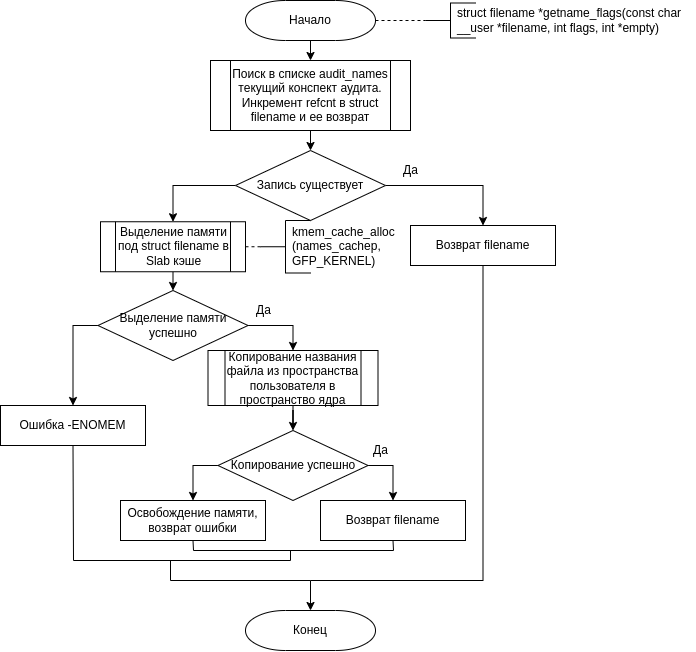
\includegraphics[scale=0.53]{assets/getname_flags.png}
	\end{center}
	\caption{Схема алгоритма функции getname\_flags()}
\end{figure}

\begin{figure}[H]
	\begin{center}
		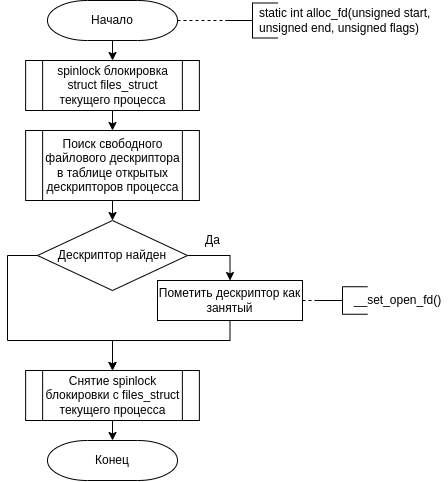
\includegraphics[scale=0.52]{assets/alloc_fd.png}
	\end{center}
	\caption{Схема алгоритма функции alloc\_fd()}
\end{figure}

\begin{figure}[H]
	\begin{center}
		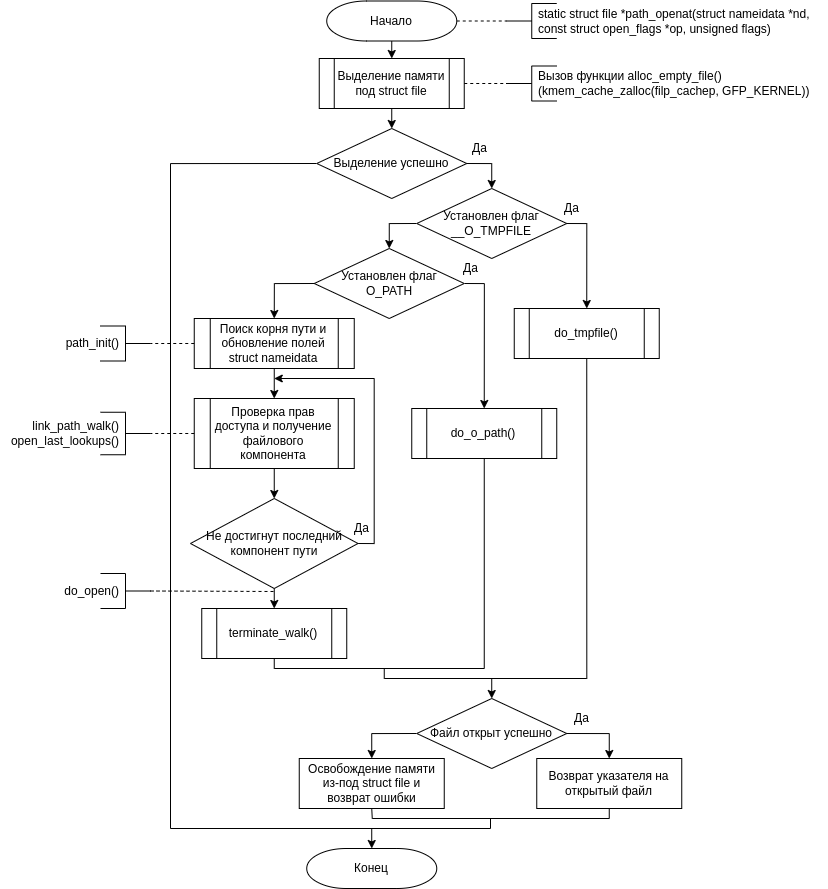
\includegraphics[scale=0.52]{assets/path_openat.png}
	\end{center}
	\caption{Схема алгоритма функции path\_openat()}
\end{figure}

\begin{figure}[H]
	\begin{center}
		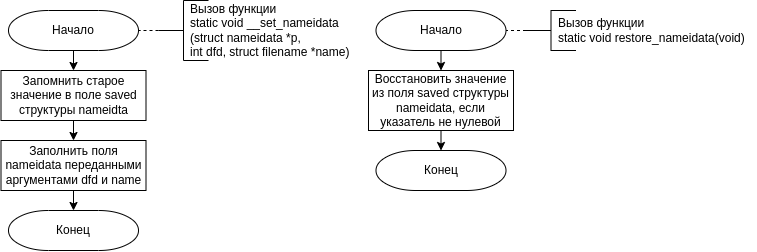
\includegraphics[scale=0.6]{assets/nameidata.png}
	\end{center}
	\caption{Схема алгоритма функций, работающих с nameidata}
\end{figure}

\begin{figure}[H]
	\begin{center}
		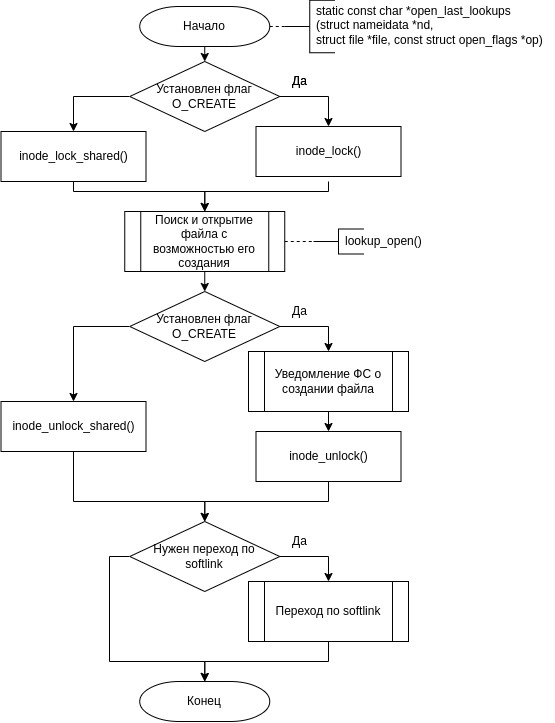
\includegraphics[scale=0.65]{assets/open_last_lookups.png}
	\end{center}
	\caption{Схема алгоритма функции open\_last\_lookups()}
\end{figure}

\begin{figure}[H]
	\begin{center}
		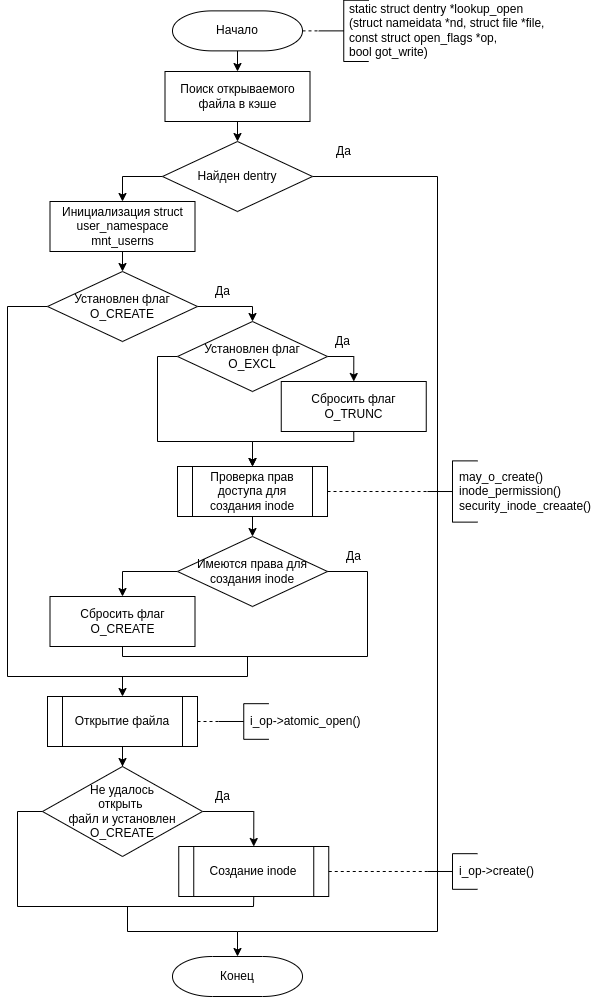
\includegraphics[scale=0.65]{assets/lookup_open.png}
	\end{center}
	\caption{Схема алгоритма функции lookup\_open()}
\end{figure}

\end{document}